\chapter{Learning to Estimate Depth from a Single Image}
\label{chapter:3D_learning_from_single_image}

\section{Introduction}

In the previous chapters we studied the image formation process and how to estimate the three-dimensional (3D) scene structure from images. We used the mathematical formulation of perspective projection, together with some hypothesis, in order to recover the missing third dimension: we could use multiple images or a single image using the rules of single view metrology.

There are many other cues that we have ignored that also inform us about the 3D structure of the scene. Instead of building precise models of how to integrate them, here we will describe a learning-based approach that bypasses modeling and instead learns from data how to recover the 3D scene structure from a single image. We will formulate depth estimation as a regression problem.

The trick consists in how to get the training data. We will discuss supervised and unsupervised methods. But before that, let's revise what cues are present in single images that reveal the 3D scene structure.

\section{Monocular Depth Cues}

Before delving into the subject of this chapter, let's quickly review some of the image features that are used by the human visual system to interpret the 3D structure of a picture. \marginnote{For a greater understanding of depth cues, take an art class.}

{\bf Shading}\index{Shading} refers to the changes in image intensity produced by changes in surface orientation. The amount of light reflected in the direction of the viewer by a surface illuminated by a directional light source is a function of the surface albedo, the light intensity, and the relative angle between the light direction and the surface normal orientation, as we discussed in \sect{\ref{sec:light_interacting_with_surfaces}}. {\bf Shape from shading}\index{Shape from shading} \cite{Barron2015ShapeIA,Freeman90d,Horn89a,Pentland90} studies how to recover shape by inverting the rendering equations.

Another source of 3D information are {\bf texture gradients}\index{Texture gradients}. As far things appear smaller than closer things, by measuring the relative size between textural elements that appear in different image regions we can get a coarse estimate of the 3D scene structure (see \fig{\ref{fig:aerial_perspective}}[a]). Many methods using texture gradient cues have been proposed over time \cite{Witkin81}.

Another source of information about the 3D scene structure are shadows and interreflections. We saw in \chap{\ref{chap:looking_at_images}}, \fig{\ref{fig:cues_for_suppport}} an example of how interreflections can inform us about the location of a ball. The use of shadows and interreflections by the human visual system has been the focus of lots of studies \cite{Knill97,Madison2001}. There are also computational approaches that use shadows and interreflections to recover 3D \cite{Nayar1991,Karnieli2022}.

When looking at large landscapes, like a mountain range, mountains that are far away have lower contrast due to dispersion by the atmosphere (see \fig{\ref{fig:aerial_perspective}}[b]). This effect gets accentuated when there is fog. Therefore, contrast can be used as a cue to infer relative distances between objects. This depth cue is called {\bf aerial perspective}\index{Aerial perspective} or atmospheric perspective. One example using haze to infer depth is in \cite{Kaiming2009}.


\begin{figure}
    \centerline{
        \sublabel{a}{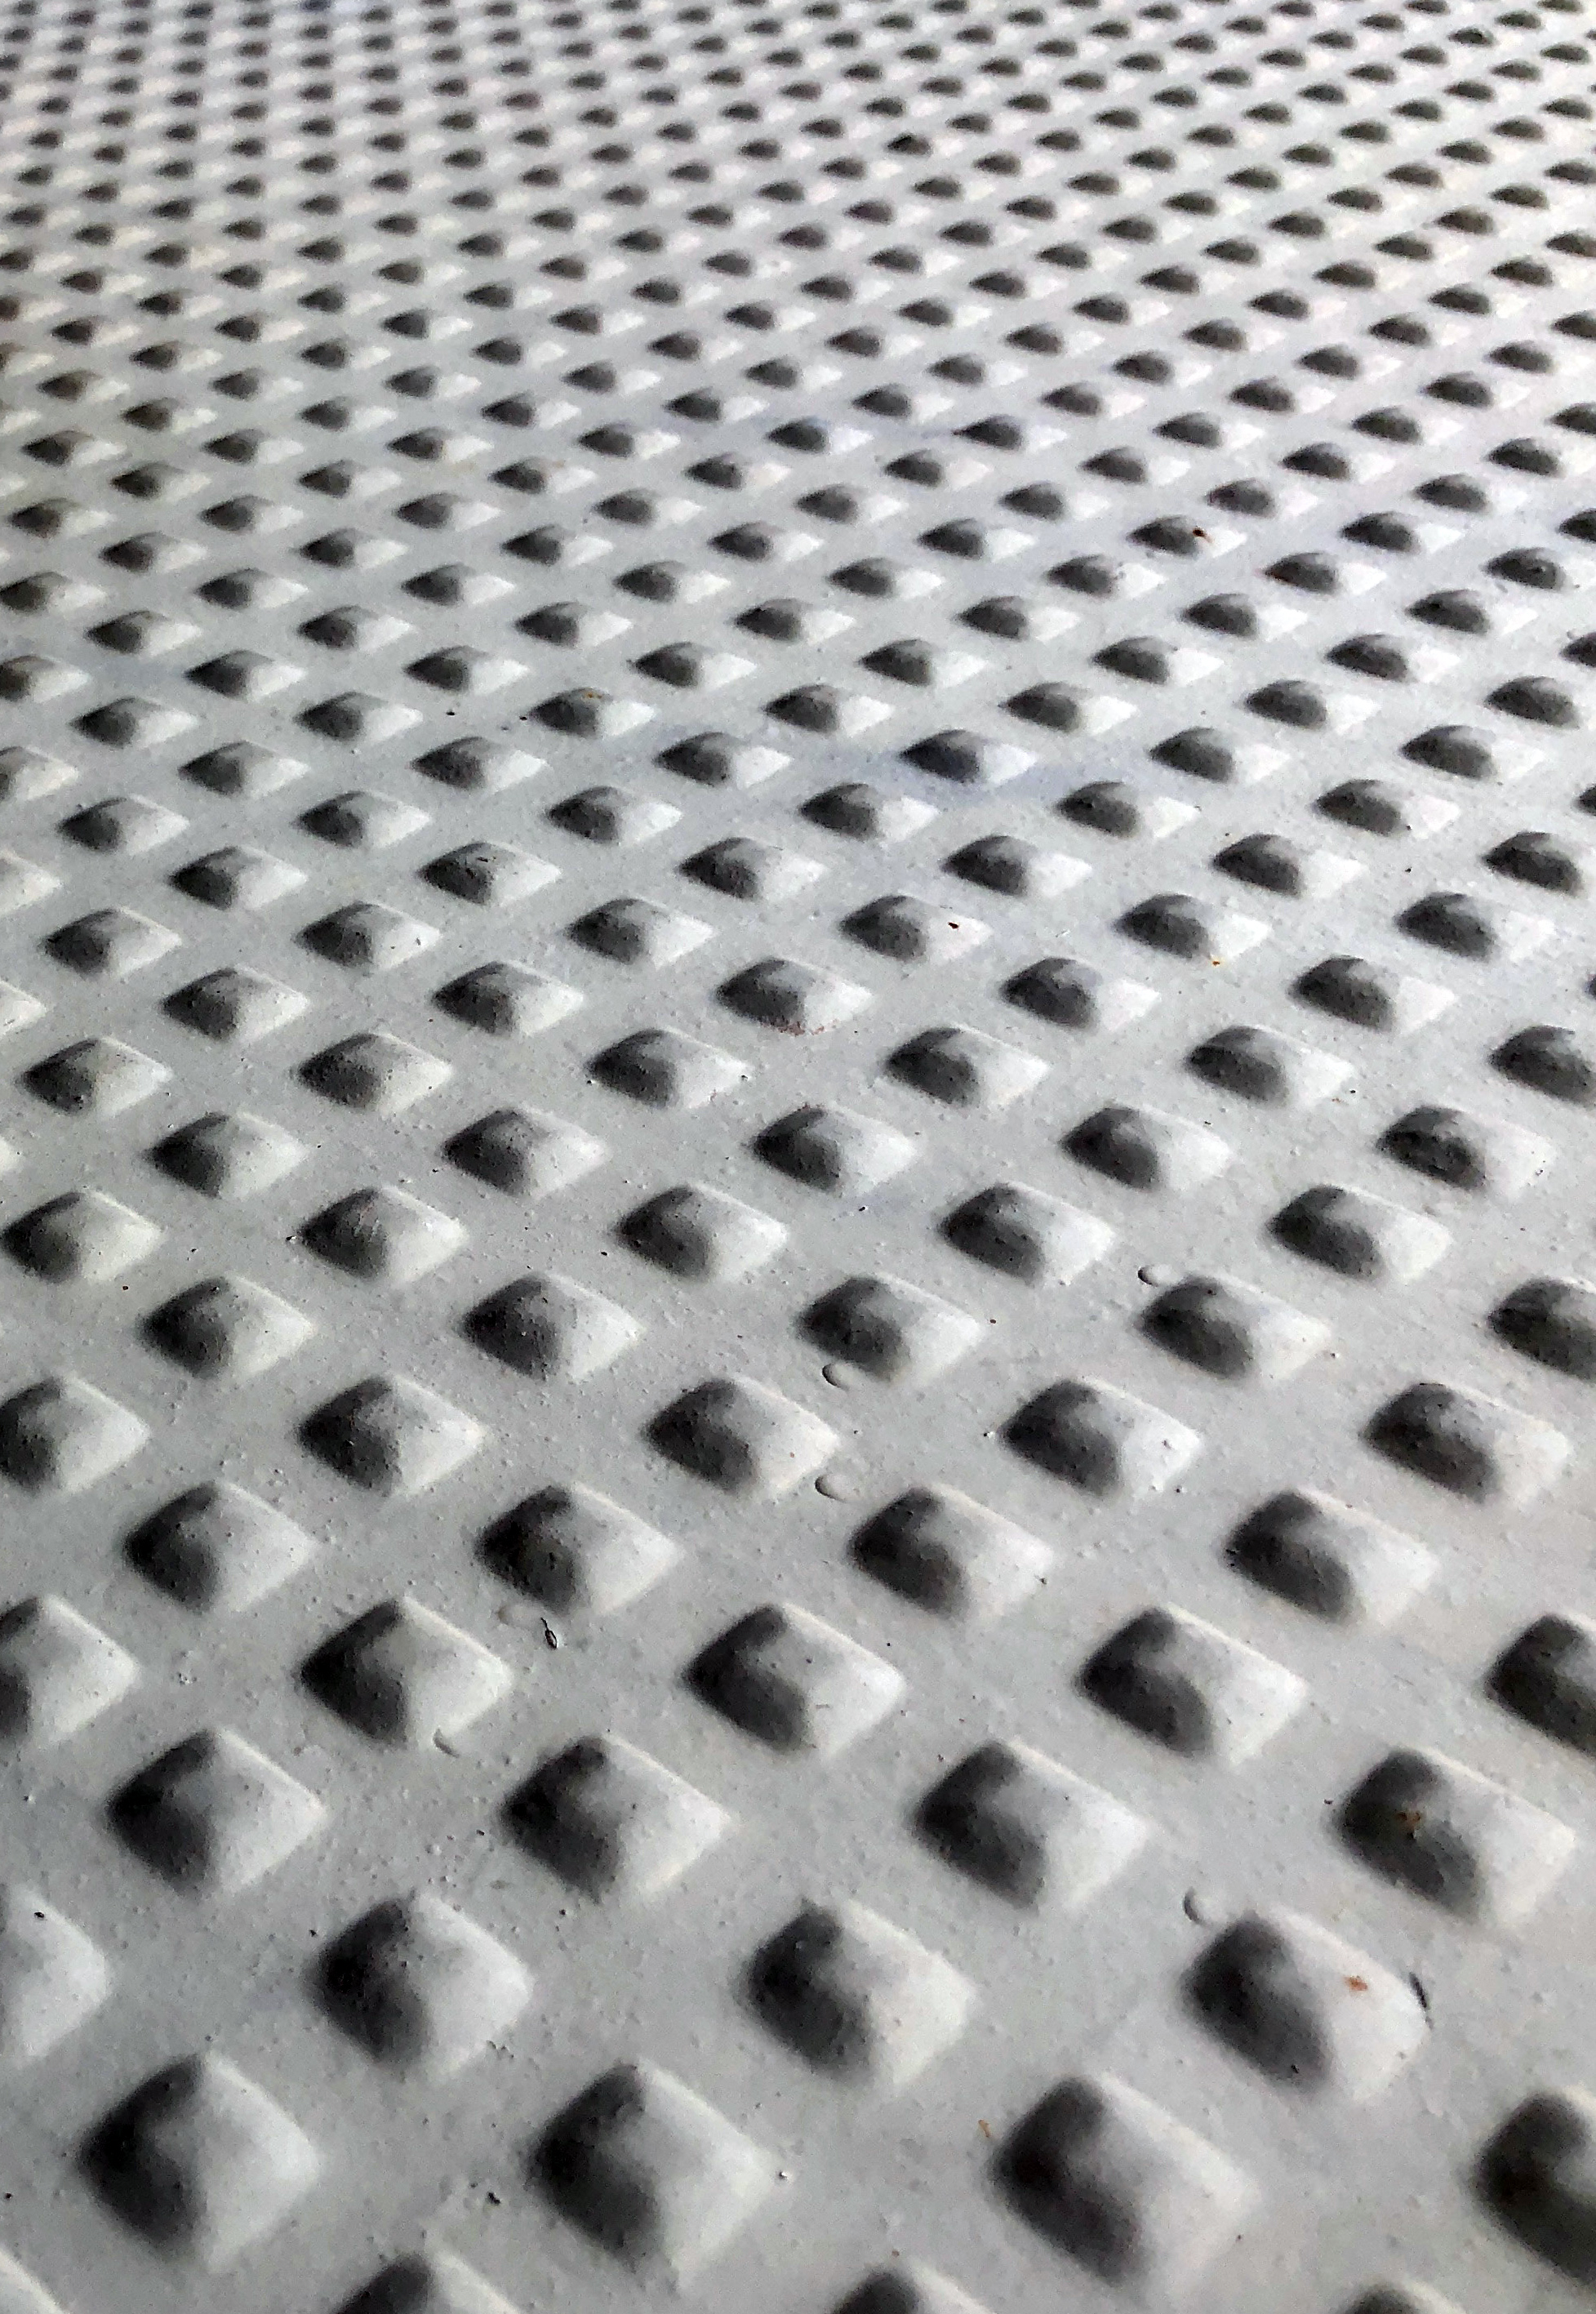
\includegraphics[height=.53\linewidth]{figures/learning_3d/IMG_0508.JPG}}
        \sublabel{b}{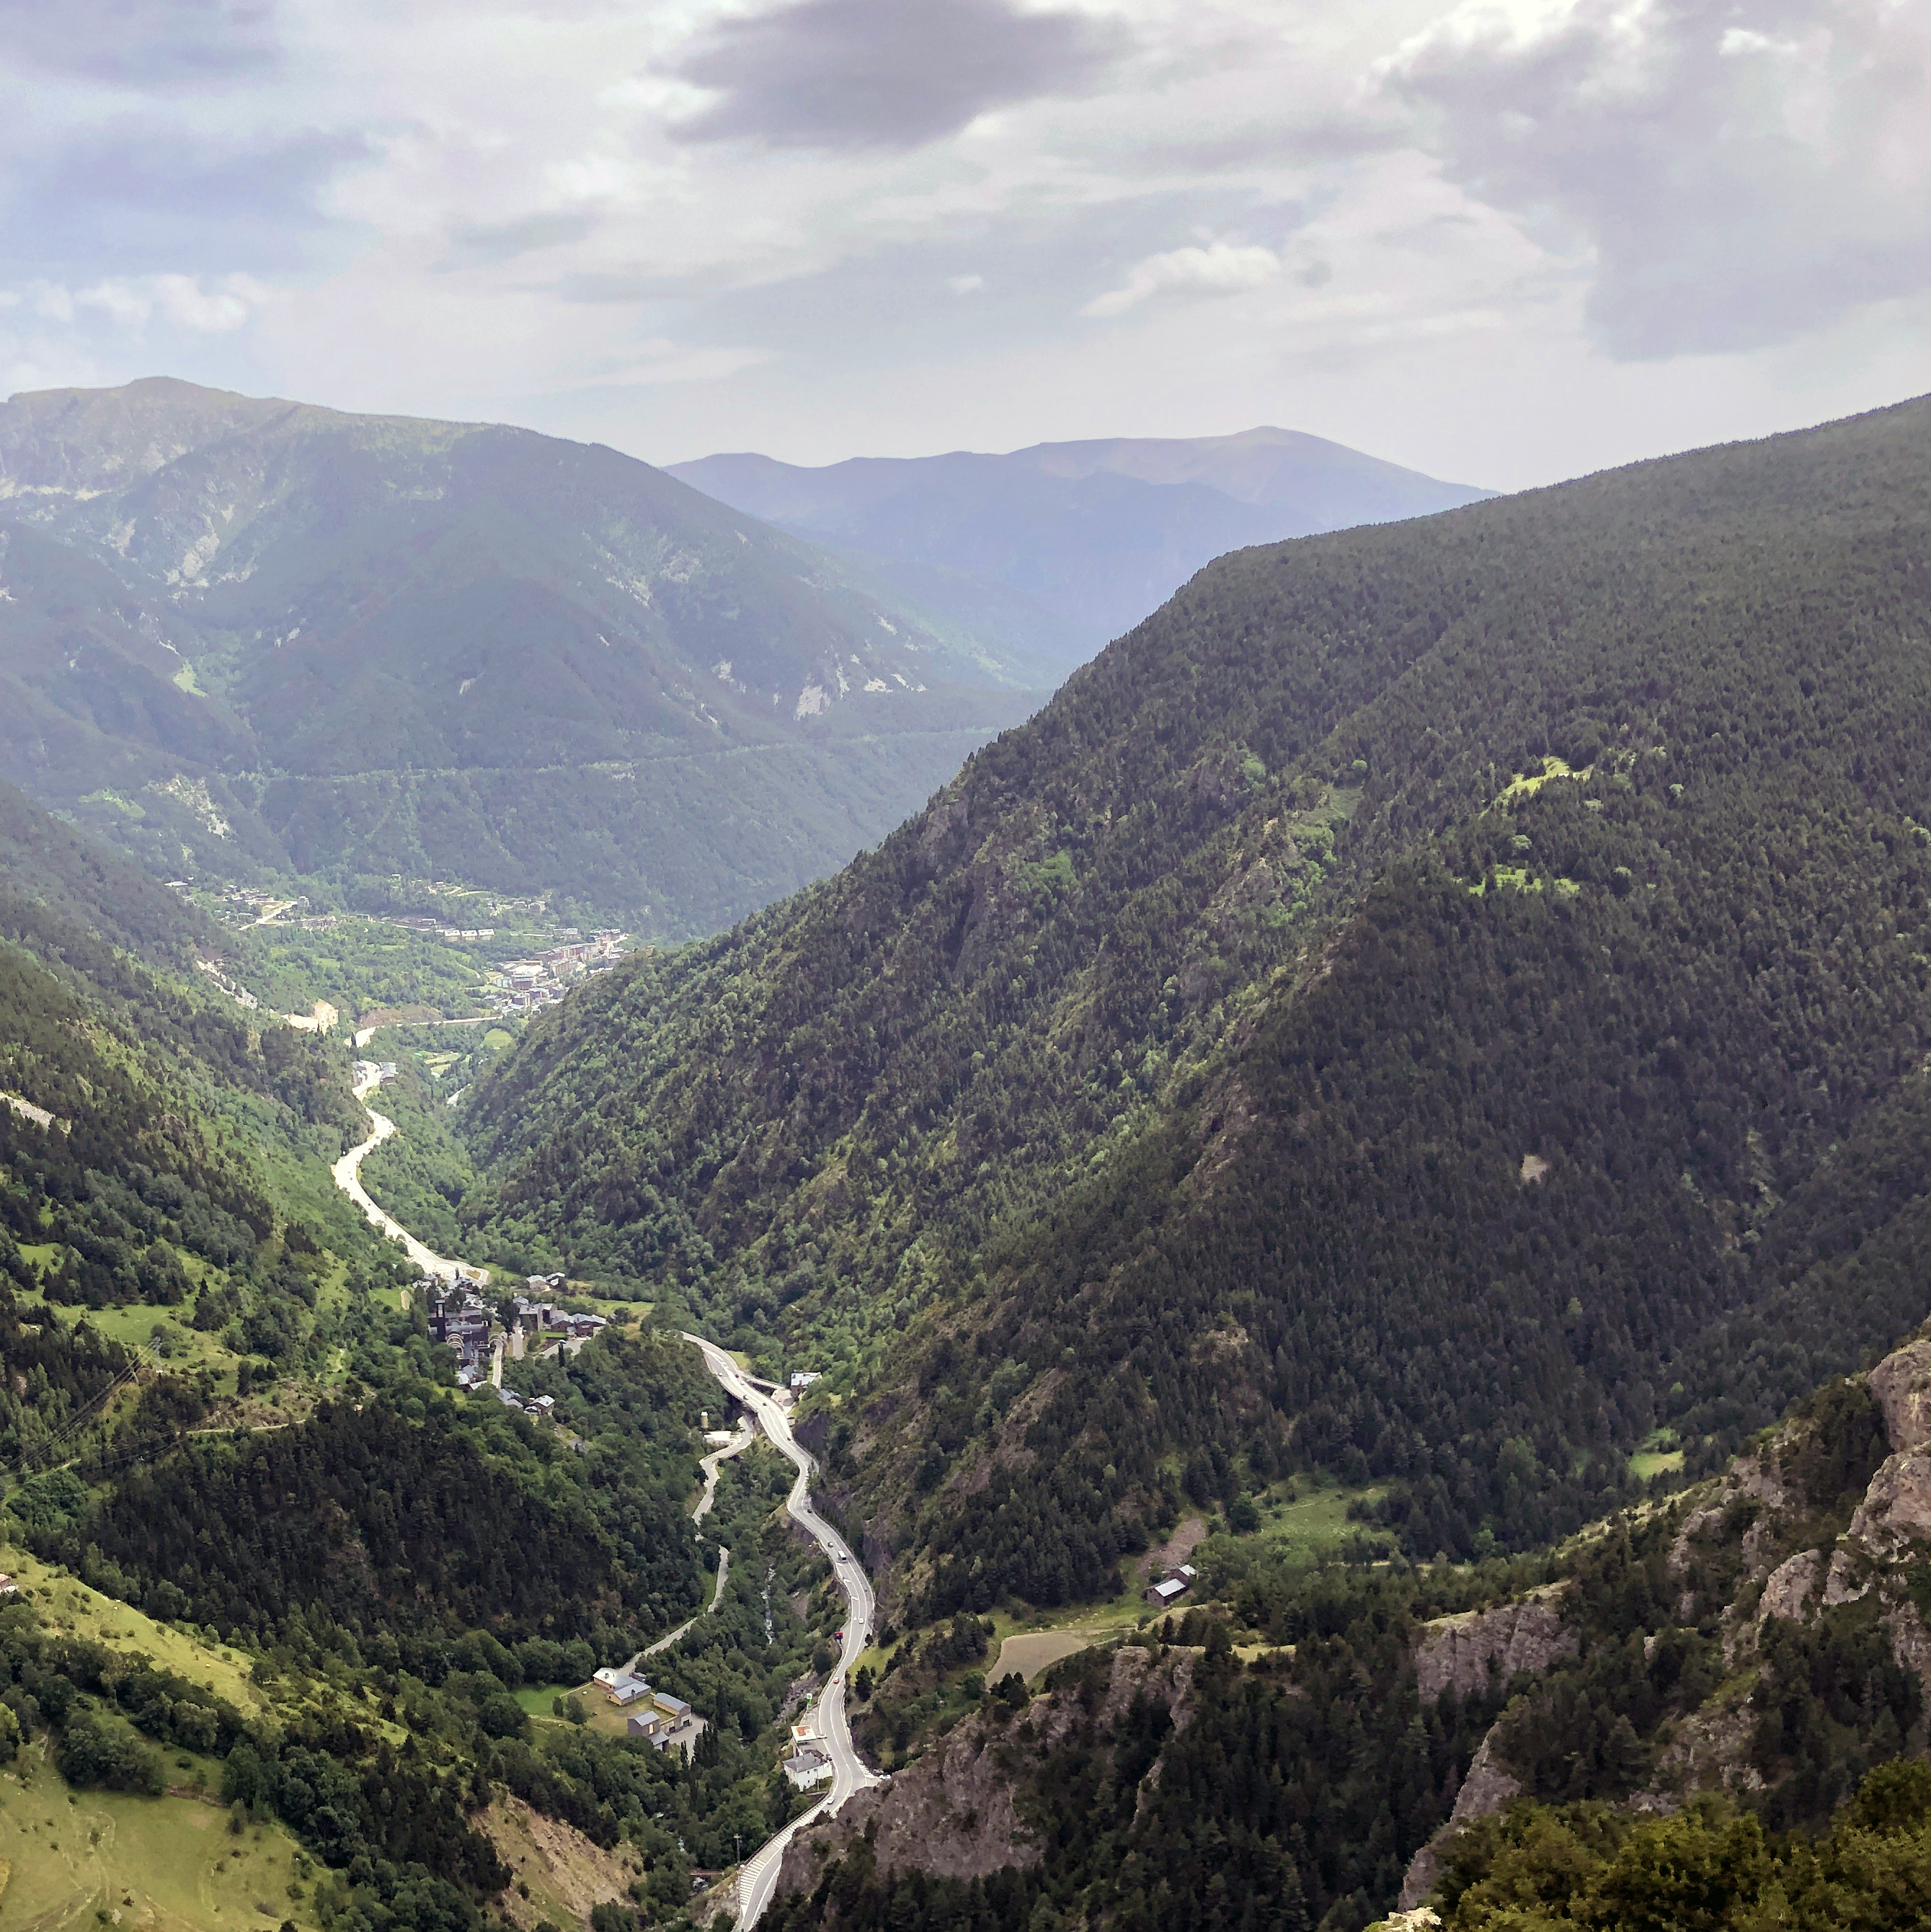
\includegraphics[height=.53\linewidth]{figures/learning_3d/IMG_2772_crop.jpg}}
    }
    \caption{(a) This image contains multiple 3D cues: shading effects (bump shapes), texture gradients (relative size between bumps), and linear perspective (due to the regular arrangement of the bumps). (b) Aerial perspective. Objects far in the background have lower contrast than objects closer to the camera.}
    \label{fig:aerial_perspective}
\end{figure}

Depth can also be estimated by detecting {\bf familiar objects} with known sizes. One example is people detection. Objects with known sizes can be used to estimate absolute depth while many of the cues that we discussed before can only give relative depth measurements. One example of using object sizes to reason about 3D geometry is \cite{Hoiem2008}.

And finally, {\bf linear perspective} provides strong cues for 3D reconstruction as we already studied in \chap{\ref{chapter:3D_single_view}}.





\section{3D Representations}

When thinking about learning based approaches, it is always good to question the representation for the input and the output. Choosing the right representation can dramatically impact the performances of the final system (even when using the same training set and the same architecture). 3D information can be represented in many different ways (i.e., disparity maps, depth maps, planes, 3D point clouds, voxels, implicit functions, surface normals, meshes) and there are methods for each one of those representations.

%\subsection{From depth maps to point clouds}
%~\\


In the rest of this chapter we will use depth maps (or disparity maps which is related to the inverse of the depth as we saw in \chap{\ref{chap:stereo_vision}}.

Most depth sensors capture aligned RGB images, $\img [n,m]$, and dense depth maps, $z [n,m]$, as shown in \fig{\ref{fig:kinect}}. Given a dense depth map, we can translate the depth into a 3D point cloud if we know the intrinsic camera parameters, $\mathbf{K}$, of the sensor.



\begin{figure}[t]
    \centerline{
        \sublabel{a}{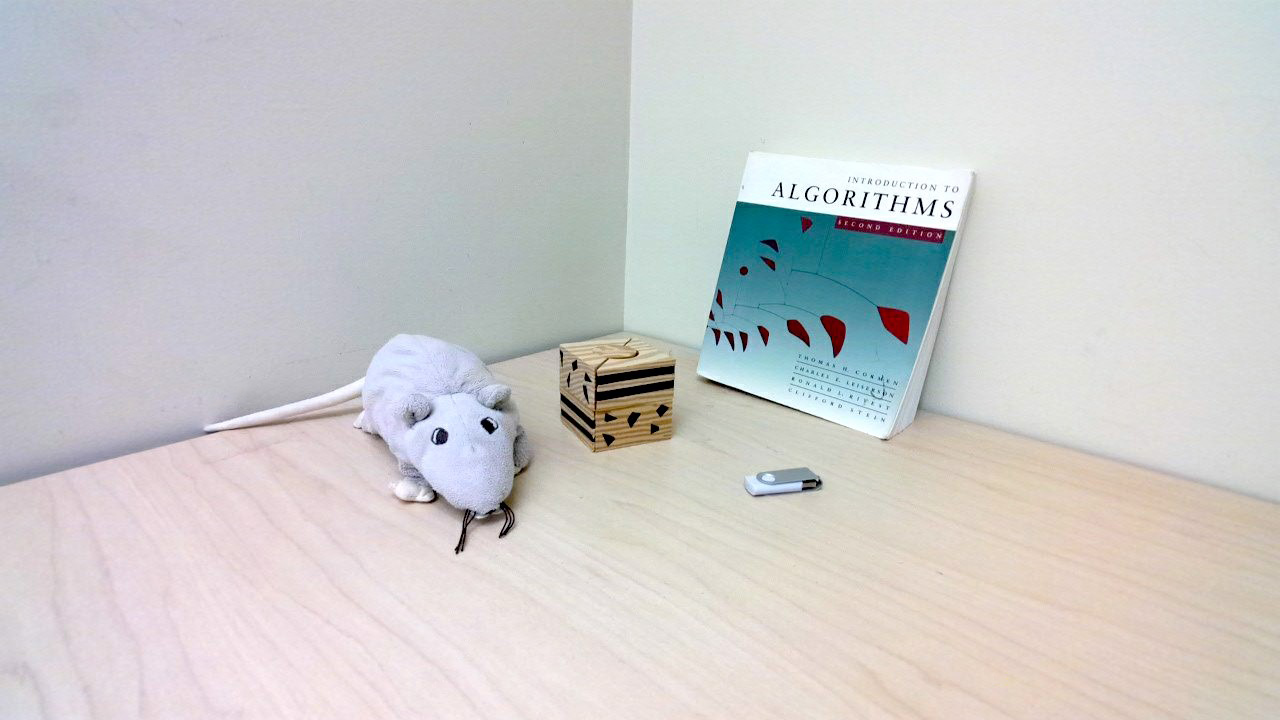
\includegraphics[width=.475\linewidth]{figures/learning_3d/rgb.jpg}}
        \sublabel{b}{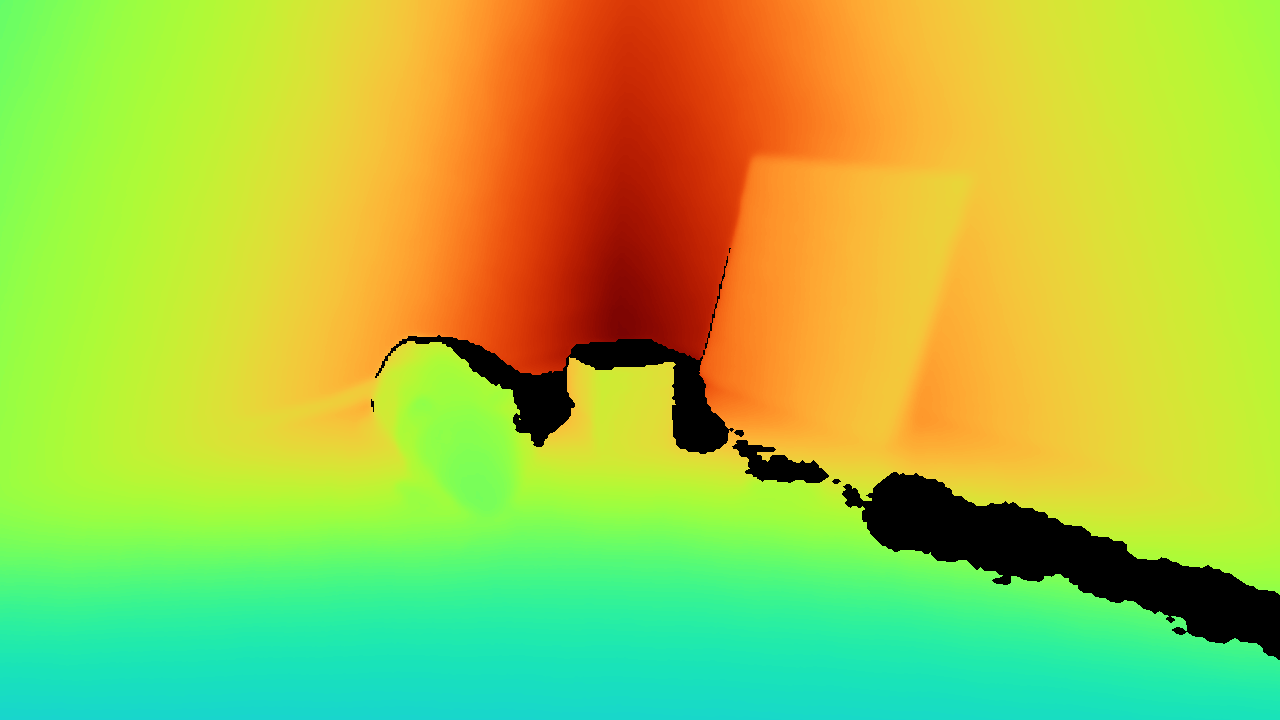
\includegraphics[width=.475\linewidth]{figures/learning_3d/depth-turbo.png}}
    }
    \caption{Image and depth captured by an Azure Kinect sensor. (a) RGB image; and (b) corresponding dense depth map. Both images have the same size of 1280 $\times$ 720 pixels.}
    \label{fig:kinect}
\end{figure}



\marginnote{Depth maps are usually visualized using the {\bf turbo colormap}, which is a modification of the {\bf jet colormap} from Matlab. We will use this convention as it differentiates a depth map from a natural gray-scale image.
    \\[6pt]
    \centerline{\includegraphics[width=.5\linewidth]{figures/learning_3d/colorbar_transposed.eps}}
    \\[6pt]
    The jet colormap can be problematic as it has a nonmonotonic intensity profile as can be seen above.
}

\Fig{\ref{fig:kinect2}} illustrates how the depth map translates into a point cloud where each pixel is mapped to a 3D point.



\begin{figure}[t]
    \centerline{
        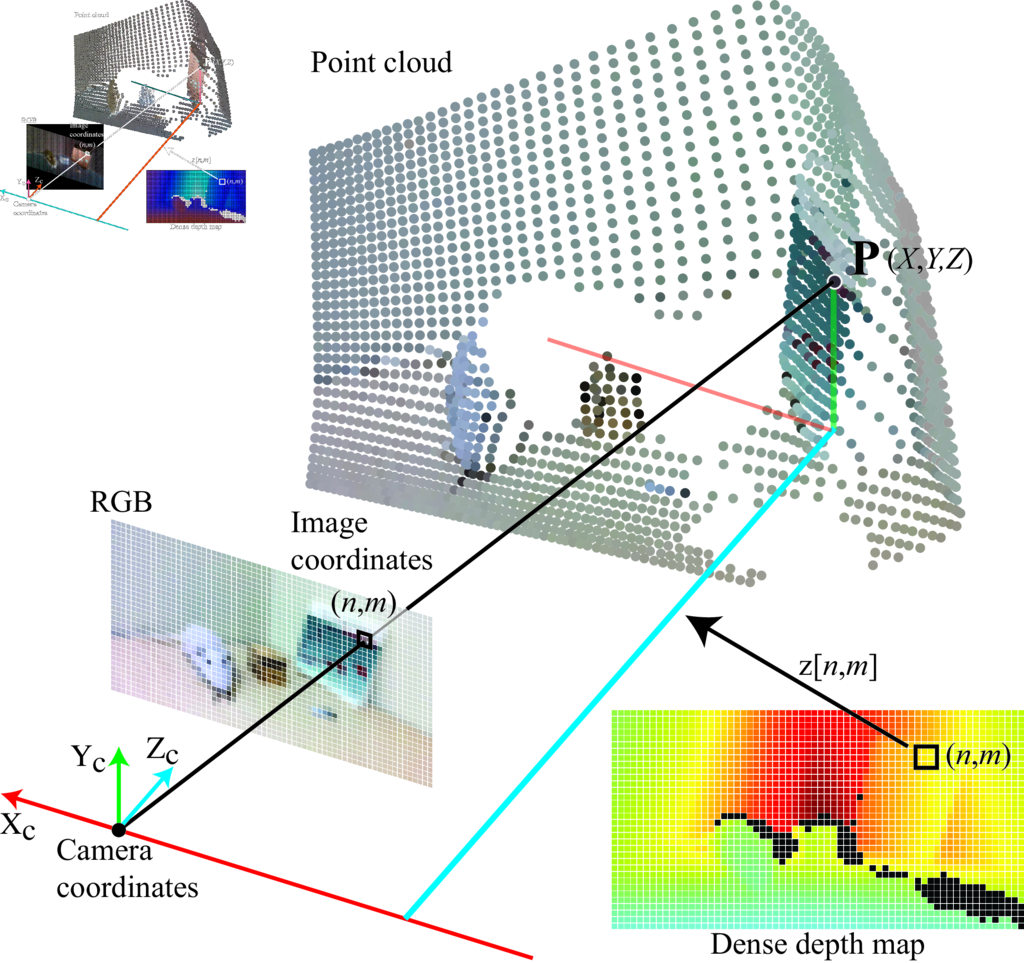
\includegraphics[width=1\linewidth]{figures/learning_3d/from_depthmap_2_pointcloud.eps}
    }
    \caption{Translating the depth map into a point cloud. This requires a calibrated camera (i.e., knowing the intrinsic camera parameters). The sketch shows how one pixel $(n,m)$ is mapped into a 3D point, $\mathbf{P}$, by using the depth, $z[n,m]$, at that location. Colored lines are parallel to the respective axis direction in the camera coordinates system.}
    \label{fig:kinect2}
\end{figure}

Using homogeneous coordinates, the equation translating a depth map into a 3D point cloud is (for each pixel):
\begin{equation}
    \mathbf{P} = z(\mathbf{p}) \mathbf{K}^{-1} \mathbf{p}
    \label{eq:3dcloudpointfromz}
\end{equation}
where $\mathbf{p}$ are the pixel coordinates of a point, $z(\mathbf{p})$ is the depth measured at that location, and $\mathbf{P}$ are the final 3D point coordinates.
In heterogeneous coordinates, and making the pixel locations explicit, \eqn{\ref{eq:3dcloudpointfromz}} can be rewritten as:
\begin{eqnarray}
    X[n,m] &=& \left( n-c_x \right) \frac{z[n,m]}{a} \nonumber \\
    Y[n,m] &=& \left( m-c_y \right) \frac{z[n,m]}{a} \nonumber \\
    Z[n,m] &=& z[n,m]
\end{eqnarray}
where $a$, $c_x$ and $c_y$ are the intrinsic camera parameters (in pixel units). This writing shows that the 3D point coordinates are three images $X[n,m]$, $Y[n,m]$, and $Z[n,m]$ with the same size as the input image.

In a point cloud, there is no notion of grouping of 3D points. 3D points are isolated and are not connected to each other. Note that translating a depth map (or a point cloud) into a mesh requires solving the perceptual organization problem first. A mesh connects points with triangles, but only makes sense to connect points that belong to the same surface or that are in contact.



%\section{Learning based methods}
\section{Supervised Methods for Depth from a Single Image}

Previous computer vision approaches for 3D reconstruction from single images focused on developing the formulation to extract depth using one or few of the cues we discussed in the previous section, and can only be applied to a restricted set of images. Learning-based methods instead have the potential to learn to extract many cues from images, decide which cues are more relevant in each case, and combine them to provide depth estimates. There were a number of early models that applied learning for recovering 3D scene structure \cite{Saxena2008,Derek2005} but in this chapter we will focus on methods using deep learning although the approaches described here are independent of the particular learning architecture used.


In the supervised setting we will assume that we have a training set that contains $N$ images, $\img^{(i)} [n,m]$, and their associated depth maps, $z^{(i)} [n,m]$. In this formulation, depth estimation becomes a pixelwise regression problem. Usually $\mathbf{z}^{(i)}$ and $\boldimg^{(i)}$ are images of the same size.
Our goal is to estimate depth at each pixel, $\hat{z}^{(i)}[n,m]$, from a single image using a learnable function, $h_\theta$:
\begin{equation}
    \hat{\mathbf{z}}^{(i)} = h_\theta \left( \boldimg^{(i)} \right)
\end{equation}
where the parameters $\theta$ are learned by minimizing the loss over a training set:
\begin{equation}
    \theta^* = \argmin_{\theta} \frac{1}{N}\sum_{i=1}^N \mathcal{L} \left( \hat{\mathbf{z}}^{(i)}, \mathbf{z}^{(i)} \right)
\end{equation}



\subsection{Collecting Training Data}

Coming up with efficient and scalable data collection strategies is crucial in this task. Several methods for supervised learning from single images differ mostly on how they collect the data. This simplest data capture method is using a depth sensor such as an RGB-D camera or a light detection and ranging (LiDAR) device.
\marginnote{LiDAR (Light Detection and Ranging) is a device that calculates distances by measuring the time taken for emitted light to return after reflecting off a surface (time of flight).
    A liDAR produces a range image by scanning multiple direction. The output is a point cloud.}
Two examples of datasets are the NYUv2 dataset \cite{SilbermanECCV12}, captured using a handheld Microsoft Kinect sensor while walking indoors, and the KITTI dataset \cite{Geiger2013}, collected from a moving vehicle with a LiDAR scan.

Other methods consist of using stereo pairs for training \cite{Xian2018} or multiview geometry methods that provide more accurate 3D estimates. MegaDepth \cite{MegaDepthLi18} uses scenes captured with multiple cameras to get good 3D reconstructions using structure from motion techniques. This allows creating a dataset of images and associated depth maps that can be used to train depth from single image methods.


\subsection{Loss}

Once we have a dataset, the next steps consist in using an appropriate loss to optimize the parameters of the depth estimator. One simple loss is the L2 loss between the estimated depth, $\hat{\mathbf{z}}$ and the ground truth depth, $\mathbf{z}$.

\begin{equation}
    \mathcal{L} \left( \hat{\mathbf{z}}, \mathbf{z} \right) =  \sum_{n,m} \left( \hat{z}[n,m] - z[n,m] \right) ^2
\end{equation}
This loss assumes that it is possible to estimate the real depth of each point, which might not be possible in general due to the scale ambiguity. Often, depth may only be estimated up to a global scaling factor. The {\bf scale-invariant loss}\index{Scale-invariant loss} addresses this by eliminating the global scale factor from the calculation:
\begin{equation}
    \mathcal{L} \left( \hat{\mathbf{z}}, \mathbf{z} \right) =  \sum_{n,m} \left( \hat{z}[n,m] - z[n,m] - \alpha\right) ^2
\end{equation}
where $\alpha = \frac{1}{NM} \sum_{n,m} \hat{z}[n,m] - z[n,m]$. This loss compares the estimated and ground truth depth at each pixel independently. In order to get a more globally consistent reconstruction one can also introduce in the loss the depth derivatives, although ground truth derivatives might be noisy depending on how the depth has been collected. Optimizing depth reconstruction might over emphasize the errors for points that large depth values. One way to mitigate this is to optimize the reconstruction of the log of the depth, $\log \left( z[n,m] \right)$, or the disparity, which corresponds to the inverse of the depth, $1/z[n,m]$.
A more complete set of losses are reviewed in \cite{Ranftl2021,Ranftl2022}.

%MiDaS

%scale- and shift-invariant trimmed loss that operates on an inverse depth representation

\subsection{Architecture}

%Architectures

%Estimating 3D and camera parameters with respect to the ground plane

The function, $h_\theta$, is usually implemented with a neural network as shown in \fig{\ref{fig:encoder_decoder_arch_depth}}. The architecture illustrated in the figure is a encoder-decoder with skip connections. The input is an red-green-blue (RGB) image and the output is a depth map. The architecture shown is very generic and there is nothing specific to the fact that it will be trained to uniquely estimate depth, but one could consider adding other constraints such as a preference for planar shapes, or introducing other structural priors. However, must current approaches will use a fairly generic architecture and let the data and the loss decide what the best function is.

\begin{figure}[t]
    \centerline{
        \includegraphics[width=1\linewidth]{figures/learning_3d/encoder_decoder_arch.eps}
    }
    \caption{Typical architecture for depth estimation from a single image\cite{Xian2018}. }
    \label{fig:encoder_decoder_arch_depth}
\end{figure}

Existing methods rely on training on massive amounts of data to achieve good generalization across a wide set of images. \Fig{\ref{fig:office_midas}} shows the result of applying the method from \cite{Ranftl2022} on the office scene from \fig{\ref{fig:finding_depth_office}} in the previous chapter.

\begin{figure}
    \centerline{
        \sublabel{a}{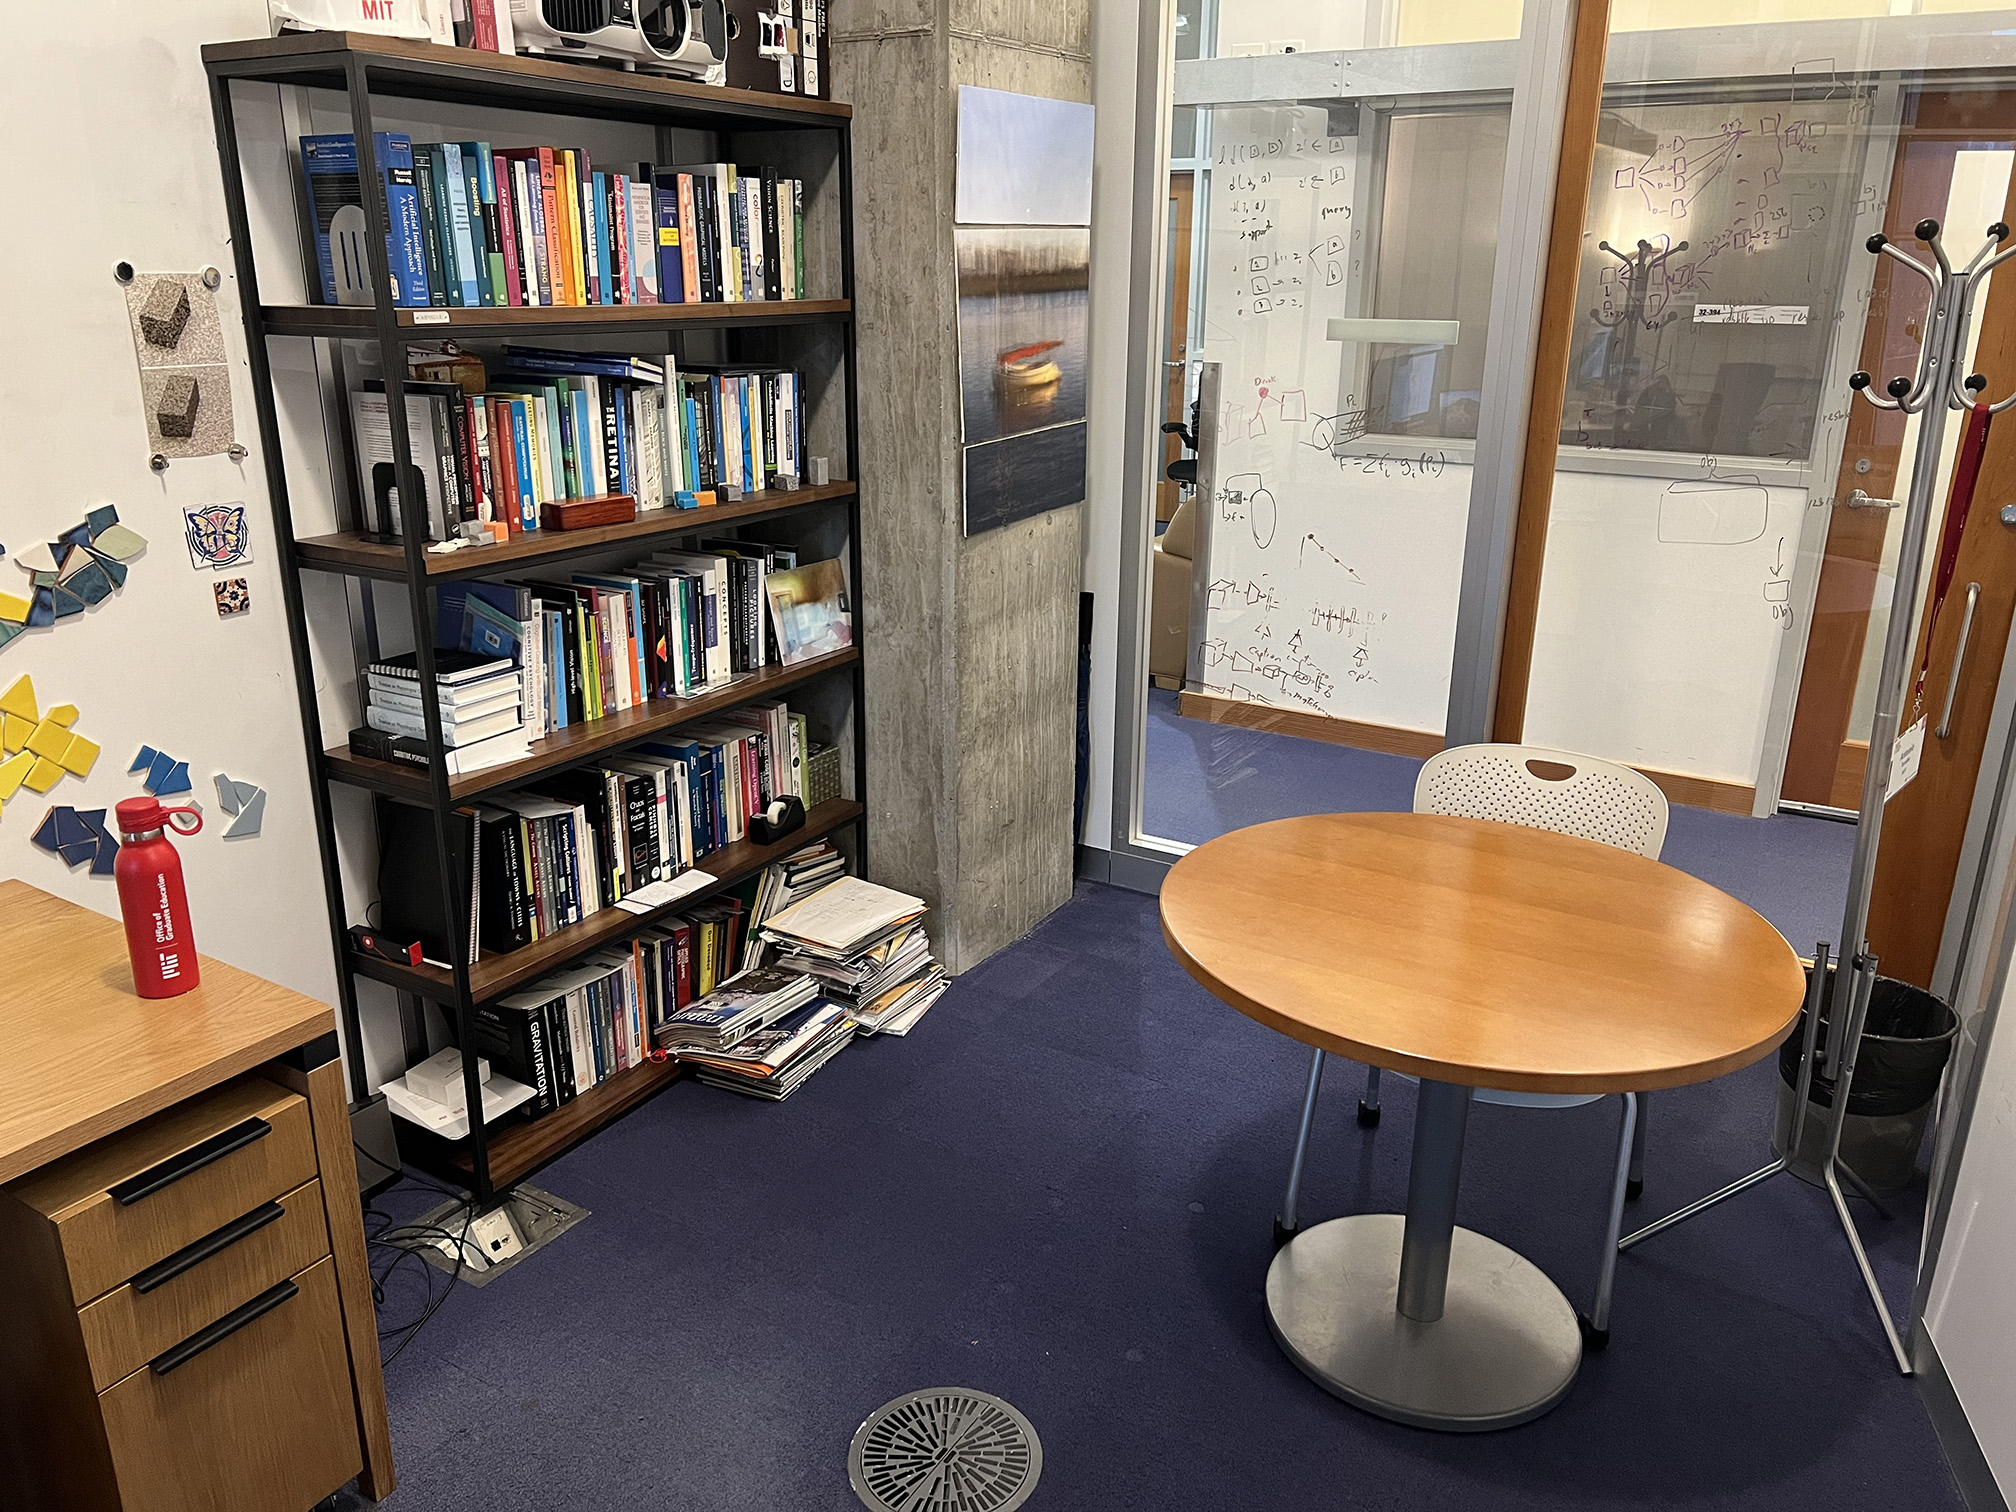
\includegraphics[height=.35\linewidth]{figures/learning_3d/IMG_6186_small.jpg}}
        \sublabel{b}{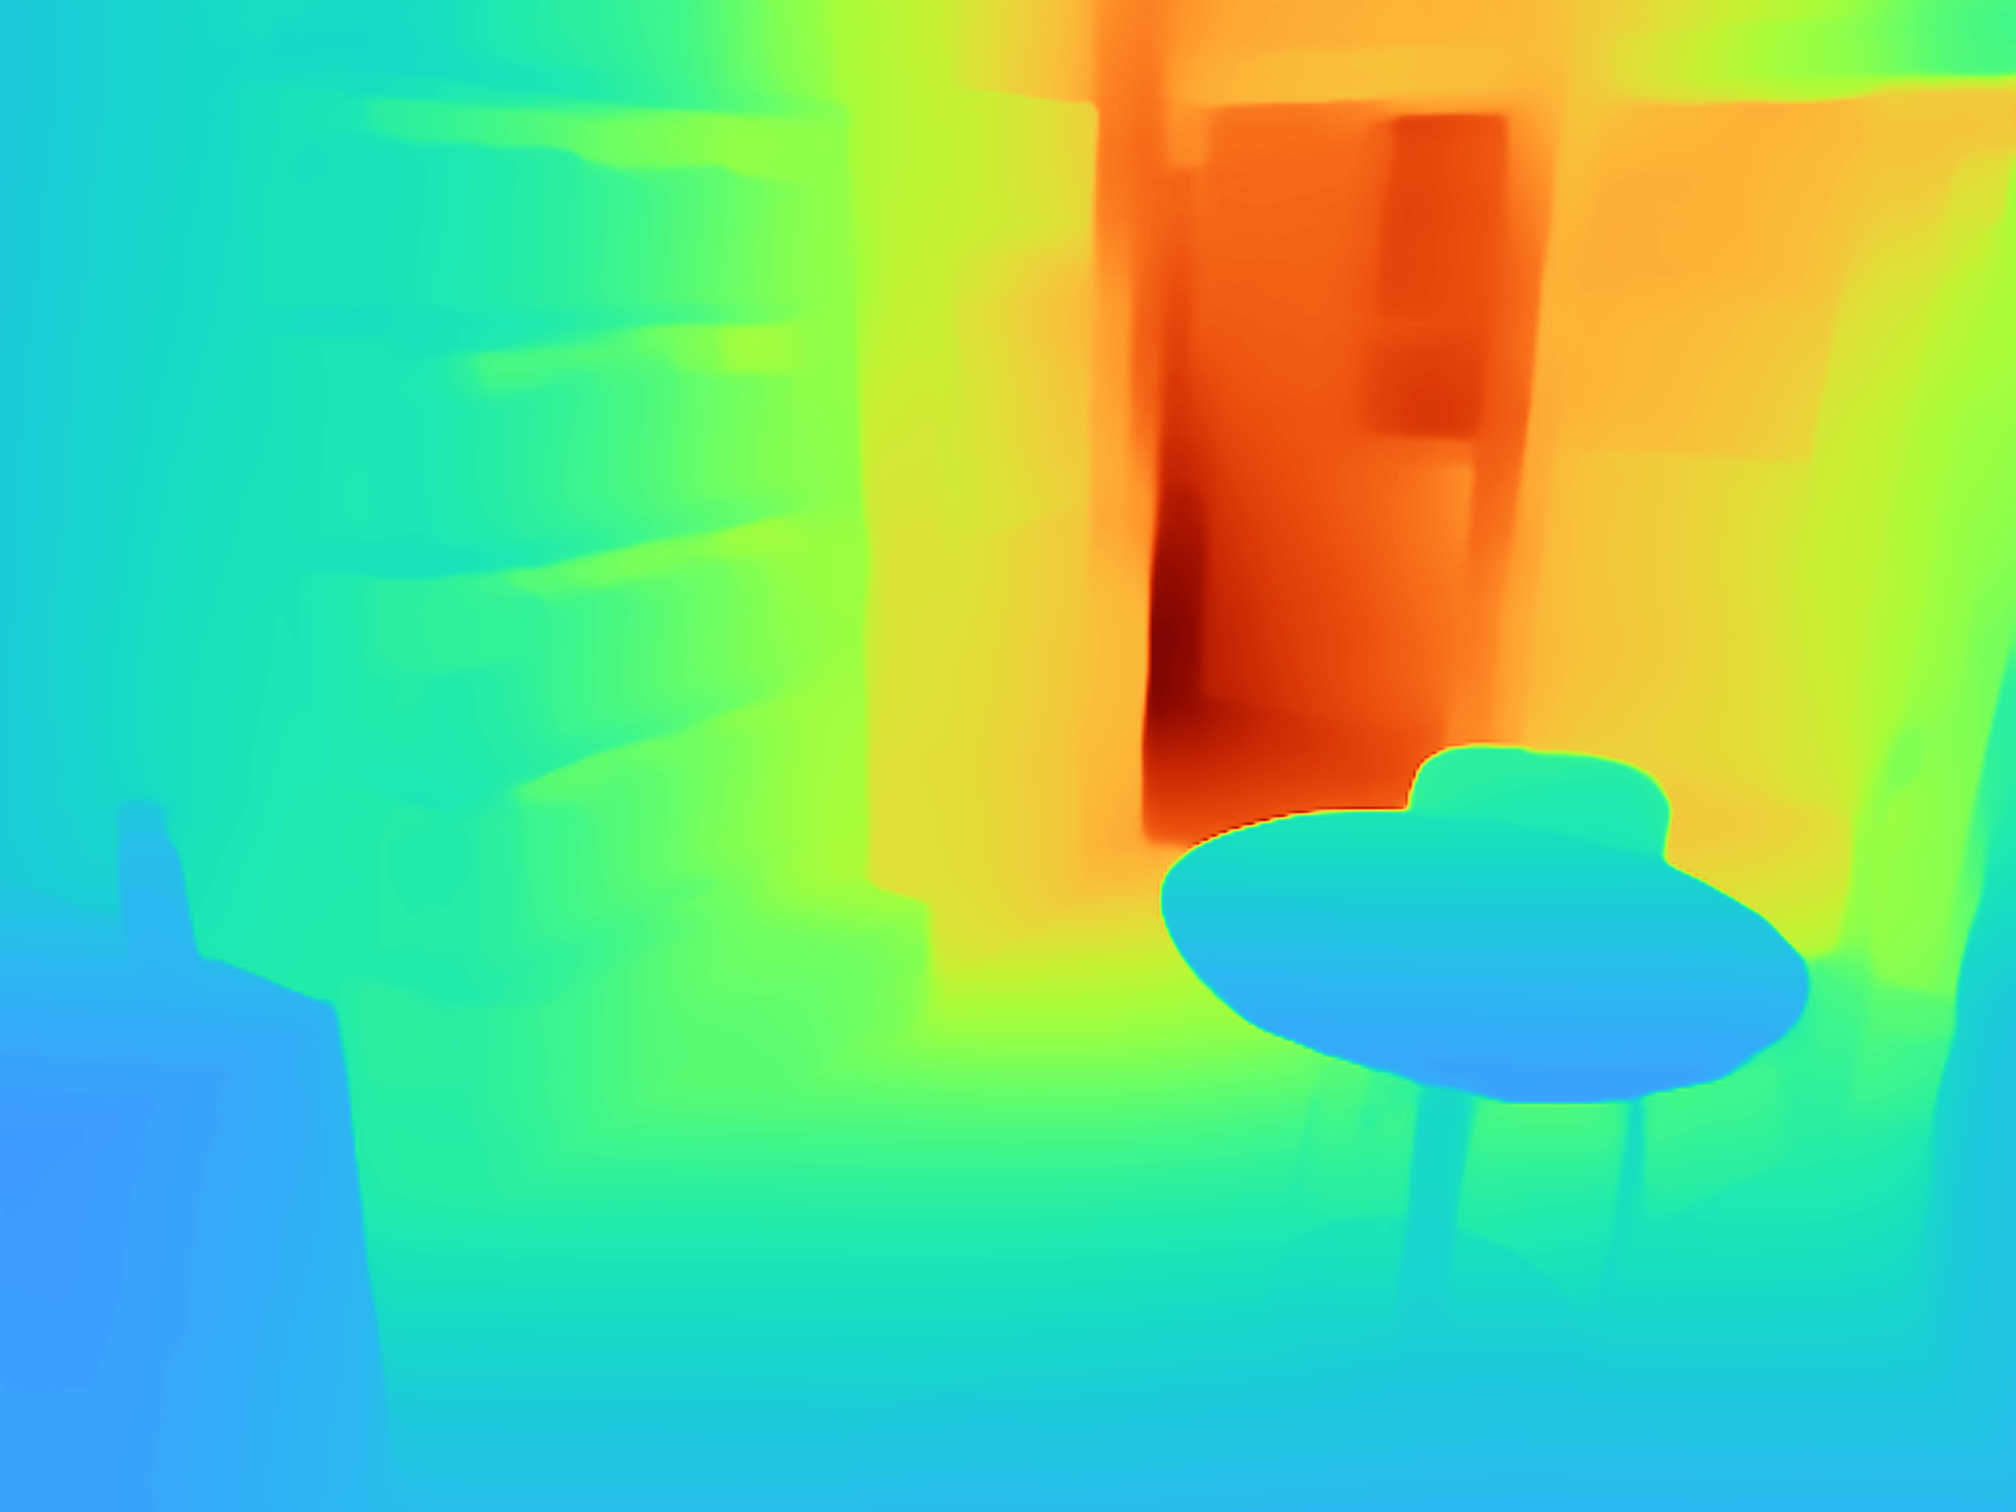
\includegraphics[height=.35\linewidth]{figures/learning_3d/Zmap_turbo.png}}
    }
    \caption{(a) Office scene. (b) Estimated $Z$ component by the approach from \cite{Ranftl2021,Ranftl2022}.}
    \label{fig:office_midas}
\end{figure}


Just looking at the depth map from \fig{\ref{fig:office_midas}}{b} might seem like the estimates are good. But it is hard to tell how good the estimation is with this visualization. The best way of appreciating the quality of a 3D reconstruction is by translating the depth map into a point cloud and then reconstructing the scene under different view points. \Fig{\ref{fig:office_midas_point_cloud}} shows two different view points for the office scene from \fig{\ref{fig:office_midas}}. Points near regions of depth discontinuities are removed to improve the clarity of the visualization. Points near depth discontinuities are often wrong and have depth values that are the average of the values on each side of the discontinuity.


\begin{figure}[t]
    \centerline{
        \sublabel{a}{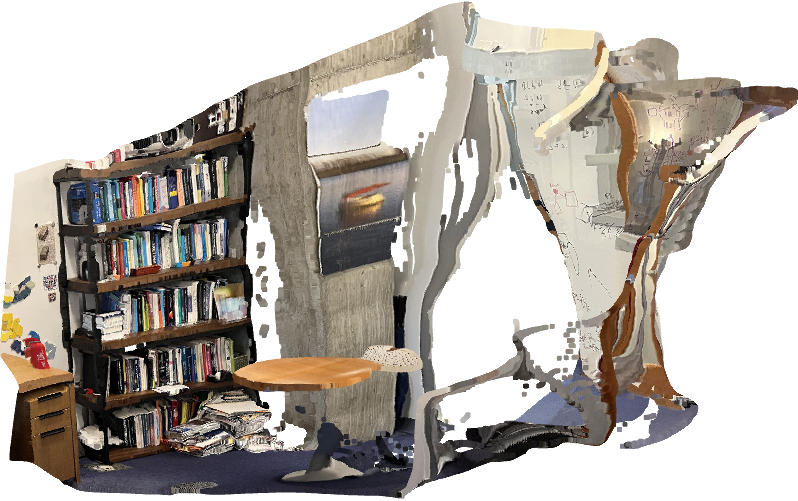
\includegraphics[height=.44\linewidth]{figures/learning_3d/view1_pointcloud.png}}
        \sublabel{b}{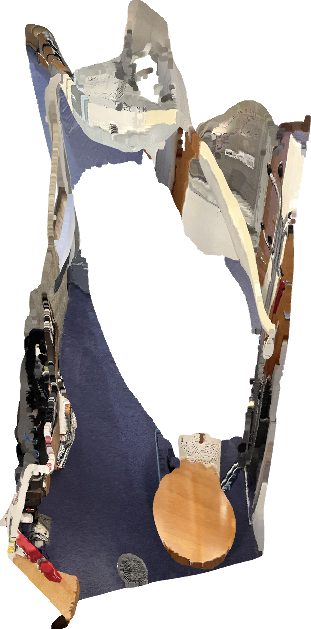
\includegraphics[height=.44\linewidth]{figures/learning_3d/view2_pointcloud.png}}
    }
    \caption{Reconstructed point cloud of the office scene with two different view points. Results are good, but not great.}
    \label{fig:office_midas_point_cloud}
\end{figure}

The point cloud has an arbitrary scaling, so we cannot directly use it to make 3D measurements. But if we are given one real distance we can calibrate the 3D reconstruction.

\marginnote{What cues are being used by a learning-based model to infer depth from a single image? What has the network learned? We discussed in  \chap{\ref{chapter:3D_single_view}} the importance of the ground plane and the support-by relationships to make 3D measurements. Is there a representation inside the network of the ground plane? Are surfaces and object represented? If you train a system, how would you try to interpret the learned representation?}

\section{Unsupervised Methods for Depth from a Single Image}

Although supervised techniques can be very effective, unsupervised techniques are more likely to eventually reach higher accuracy as they can learn from much larger amounts of data and improve over time. But unsupervised techniques pose a grander intellectual challenge: How can a system learn to perceive depth from a camera without supervision? We will assume that the camera is calibrated (i.e., the intrinsic camera parameters are known).

There are a number of approaches one could imagine. For instance, we could use some of the single view metrology techniques introduced in the previous chapter in order to generate supervisory data. A different, and likely simpler, approach would be to use motion and temporal consistency as a supervisory signal \cite{Tinghui2017}. Let's explore how this method works.

As a camera moves in the world, the pixel values between two images captured at two different time instants are related by the 3D scene structure and the relative camera motion between the two frames. Therefore, we can formulate the problem as an image prediction problem.
Let's say we have a function $f_1$ that can estimate depth from a single image, and a function $f_2$ that takes as input two frames, $\boldimg_1$ and $\boldimg_2$, and estimates the relative camera positions (the rotation and translation matrices, $\mathbf{R}$ and $\mathbf{T}$) between the two frames, as shown in \fig{\ref{fig:unsupervised_depth_system}}:
\begin{eqnarray}
    \hat{\mathbf{z}} &=& f_1(\boldimg) \\
    \left[ \hat{\mathbf{R}},\hat{\mathbf{T}} \right] &=& f_2(\boldimg_1,\boldimg_2)
\end{eqnarray}

\begin{figure}[t]
    \centerline{
        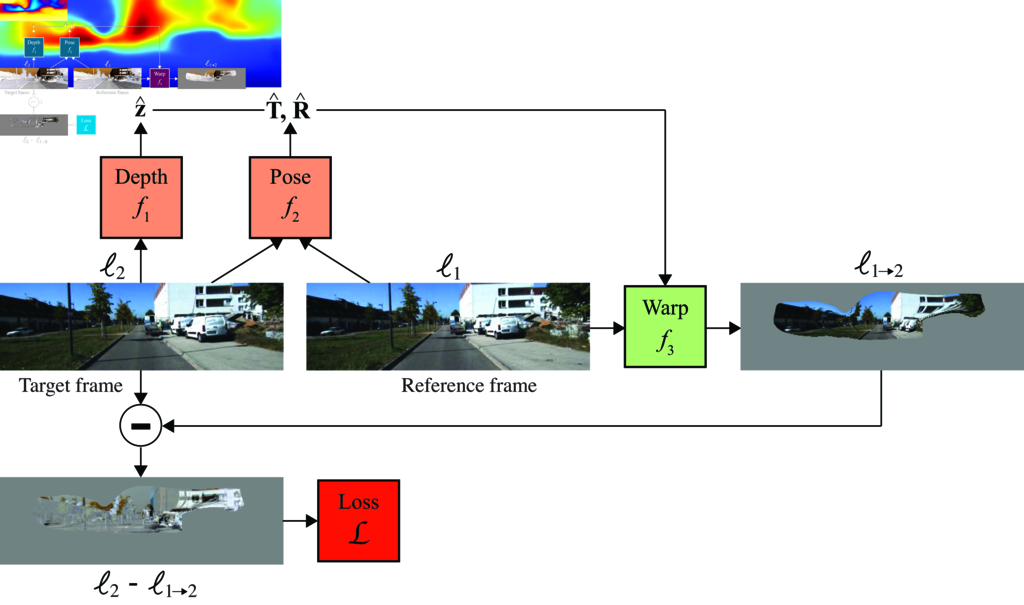
\includegraphics[width=1\linewidth]{figures/learning_3d/unsupervised_depth.eps}
    }
    \caption{System for unsupervised learning of camera motion and depth \cite{Tinghui2017}. The goal is to learn the parameters of the functions $f_1$ and $f_2$ by minimizing the reconstruction error. The function $f_3$ is deterministic.}
    \label{fig:unsupervised_depth_system}
\end{figure}


If the estimations of the depth and camera motion were correct, then we could warp the pixels in $\boldimg_1$ into the pixels of $\boldimg_2$ as depth and camera motion is all with need to precisely predict how the corresponding 3D points will move between the two frames. Warping is a deterministic function ($f_3$ in \fig{\ref{fig:unsupervised_depth_system}}) that takes as input a reference frame, the depth map, and the relative camera motion matrices and outputs an image:
\begin{equation}
    \boldimg_{1 \rightarrow 2} =
    f_3(\boldimg_1, \mathbf{z}, \mathbf{R}, \mathbf{T})
\end{equation}
The function $f_3$ is built with the tools we have studied in the previous chapters.
In \sect{\ref{sect:image_warping}} we described the procedure for warping an image using backward warping. Here we will use the same procedure.


The goal is to warp a {\bf reference frame} into a {\bf target frame}.
We want to look over all pixel locations, $\mathbf{x}$, over the target frame $\boldimg_2$, and compute the corresponding location on the reference frame $\boldimg_1$. For each pixel on the target frame, we will follow the next steps (see \fig{\ref{fig:geometry_reconstruction}} for the geometric interpretation of all the steps):
\begin{itemize}
    \item Express the image coordinates of the pixel in the target frame in homogeneous coordinates, $\mathbf{p}$.
    \item Given the depth at that location, recover the 3D world coordinates of the target point, $\mathbf{P}$. To do this we will use the intrinsic camera matrix, assumed to be known, and the depth at that point: $\mathbf{P} = z(\mathbf{p}) \mathbf{K}^{-1} \mathbf{p}$. As we do not have access to ground truth depth, we will use the function $f_1$ to estimate depth: $\hat{\mathbf{z}} = f_1(\boldimg_2)$. The coordinates of the point $\mathbf{P}$ are expressed with respect to the camera coordinates of $\boldimg_2$.
    \item We now use the camera rotation and translation matrices to change the camera coordinates to the coordinates defined by the reference frame, $\boldimg_1$. This is done as $\mathbf{P}' = \mathbf{M}\mathbf{P}$ where the matrix $\mathbf{M}$ contains the translation and rotation matrices.
    \item Finally, we project the point $\mathbf{P}'$ into the image coordinates of the reference frame $\mathbf{p}' = \mathbf{K} \mathbf{P}'$.
    \item The resulting coordinates $\mathbf{p}'$ are translated back into heterogeneous coordinates.
\end{itemize}

\begin{figure}
    \centerline{
        \includegraphics[width=.6\linewidth]{figures/learning_3d/geometry_reconstruction_12.eps}
    }
    \caption{Geometry between two images captured by a moving camera. The coordinates of corresponding points between the two frames are constrained by the 3D world coordinates of the point the relative camera motion.}
    \label{fig:geometry_reconstruction}
\end{figure}

Putting all these steps together, ignoring the transformations between homogeneous and heterogeneous coordinates, the reconstruction of $\boldimg_2$ results in:
\begin{equation}
    \img_{1 \rightarrow 2}(\mathbf{p}) =
    \img_1 \left( \mathbf{K} \hat{\mathbf{M}} \hat{z}(\mathbf{p}) \mathbf{K}^{-1} \mathbf{p} \right)
\end{equation}
where $\boldimg_{1 \rightarrow 2}$ is the result of warping image $\boldimg_1$ into $\boldimg_2$. As the coordinates of the point $\mathbf{p}'$ will not be discrete, we use bilinear interpolation to estimate the pixel value.


If the reconstruction is correct, we expect the difference $\left| \img_{1 \rightarrow 2}(\mathbf{p}) - \img_{2}(\mathbf{p}) \right|$ to be very small. There will be some errors due to pixels that are invisible in one frame but not the other, changes in illumination, or due to the presence to moving objects in the scene.

The functions $f_1$ and $f_2$ are unknown and we want to learn them in an unsupervised way. If we have very long video sequences captured with a moving camera (assuming all objects are static) we can optimize the parameters of the functions $f_1$ and $f_2$ to minimize the reconstruction error. The functions $f_1$ and $f_2$ can be neural networks and their parameters can be obtained by running back-propagation over the loss:
\begin{equation}
    \mathcal{L} =  \sum_{n,m} v\left(n,m \right) \left( \img_{1 \rightarrow 2}[n,m] - \img_{2}[n,m] \right) ^2
\end{equation}
As only the pixels with coordinates $\mathbf{p}'$ inside the image can be reconstructed by warping, we compute the loss only over the valid set of pixels. This is done using the mask $v\left(n,m \right)$, which is 1 for valid pixels and 0 for pixels that lie outside the visible part of the reference frame. The mask could also exclude pixels that fall in moving objects as those will have displacements that cannot predicted by the motion of the camera alone.

Not all camera motions provide enough information to learn about the 3D world structure. As we discussed in \chap{\ref{chapter:homography}}, if all the videos contain only sequences captured by a rotating camera, the points are related by a homography regardless of the 3D structure. Therefore, to learn depth from single images, we need to have complex camera motions inside environments with rich 3D structure.

\marginnote{To model the motion of objects we need to introduce new concepts. We will do that later when studying motion estimation in \chap{\ref{chap:optical_flow_estimation}}.}

%\begin{equation}
%KˆT _{t \rightarrow s} ˆD_t(p_t)K−1p_t
%\end{equation}




\section{Concluding Remarks}

In this chapter we have reviewed some of the key components of a system trained to estimate depth from single images. The methods are similar to other regression problems and most of the challenge consists of identifying how to collect the data needed for training. Supervised methods are more reliable than unsupervised methods for now. Unsupervised methods  rely on learning to estimate depth using the constraints present between camera motion, 3D, and photometric consistency. Unsupervised learning allow a system to learn from a very diverse set of data (as the only thing needed is video captured by a moving camera), and to adapt to new environments where ground truth supervision is not available.
